\documentclass[12pt]{article}
% \usepackage{fullpage}
\usepackage{graphics,graphicx,subfig}
\usepackage{amsmath,multicol,lscape,framed,amssymb}
\usepackage{graphicx,epic,subfig,graphicx,tikz,pifont}
%\usepackage{multirow,epic}
% \usepackage{algorithmic,algorithm}
\usepackage{hyperref,hypcap}
\usepackage{natbib}%
\usepackage{longtable}
\usepackage{textcomp}%to use \textquotesingle
% \captionsetup{type=figure}
\hypersetup{
colorlinks,%
citecolor=blue,%
filecolor=black,%
linkcolor=blue,%
urlcolor=blue,
}
\usepackage{setspace}
\bibliographystyle{chicago}

\bibstyle{plain}
\newcommand{\HRule}{\noindent\rule{\linewidth}{1.5pt}}
\newtheorem{alg}{Algorithm}
\newcommand{\cm}[1]{\begin{center}{\tt #1}\end{center}}
\newcommand{\hs}{{\tt hybrid-coal}}
\newcommand{\PP}{{\mathbb P}}


\begin{document}

\title{Hybrid-coal manual}
\author{Sha (Joe) Zhu}
\maketitle



\section{Introduction}

In phylogenetic studies, trees are used for describing evolutionary histories. In particular, a species tree presents population divergences, and a gene tree indicates the times when genes started to differentiate within populations. Even though speciation is driven by gene mutations, using a single gene tree to infer the species tree is
not ideal. Often, the inconsistency among gene trees and species trees makes describing the relationships between and among species very difficult. Common causes of the conflict include gene duplication, horizontal gene transfer, incomplete lineage sorting, and hybridization \citep{Holland2008,Meng2009}. If speciation events occur close together, it is likely that some gene copies remain the same after species divergence. This inconsistency between gene trees and species trees is referred as incomplete lineage sorting.

Hybridization refers to interbreeding between species. Offspring who carry genes from both parental species then reproduce and form a new species.
For closely related species, however, both lineage sorting and hybridization are likely to occur, e.g. an avian genus {\it Manacus} \citep{Brumfield2010} or the New Zealand alpine cicadas \citep{Buckley2006}. Here, I present research on the probabilistic modelling of coalescence with lineage sorting in hybridized species. In these models, the relationships among species are represented by a network rather than a tree, while relationships at the gene level are still represented by trees.

{\tt hybrid-coal} has been developed to calculate the gene tree probabilities within a species network.

\section{Download and installation}
{\tt hybrid-coal} can be downloaded from \url{https://github.com/hybridLambda/hybrid-coal}. Extract the source code by executing the following command:
\cm{tar -xf hybrid-coal-VERSION.tar.gz.}

It is fairly standard to compile \hs~on UNIX-like systems. In the directory {\tt hybrid-coal-VERSION}, execute the following command:
\begin{verbatim}
$./bootstrap
$make
\end{verbatim}


\section{Notation}
% \section{Notations and Input/Output formats}
%\subsection{Coalescent parameters}
%Under the coalescent process, the waiting time for lineages to coalesce is an exponential random variable. The Kingman coalescent process only allows two lineages to coalesce at a time. Thus, the mean waiting time for $b$ lineages to coalesce into $b-1$ lineages is $\binom{b}{2}$ per unit of time.

\subsection{Input/output formats}\label{coal_man:coal_input}
The input file for {\tt hybrid-coal} is a character string that describes the relationships among species. Standard Newick format is used for inputting species trees and outputting
gene trees, e.g.:
\begin{equation}
((A:t_A,B:t_B):t_{AB},C:t_C)\label{coal_man:no_root},
\end{equation}
where $t_i$ denotes the branch length from $i$ to its parent node in coalescent units.

Extended Newick formatted strings \citep{Cardona12008,Huson2010} label all internal nodes, and are used for inputting species networks. In the network string, the descendants of a hybrid node are recorded before the hybrid node the first time the hybrid node occurs; otherwise, it is written as a tip node. For example:
\begin{equation}
(((B:t_B)h\#\gamma:t^{s1}_{h},A:t_A)s1:t_{s1},(h\#\gamma:t^{s2}_{h},C:t_{C})s2:t_{s2})r,\label{coal_man:ext_no_root}
\end{equation}
where $\#$ identifies the hybrid node.
\begin{center}
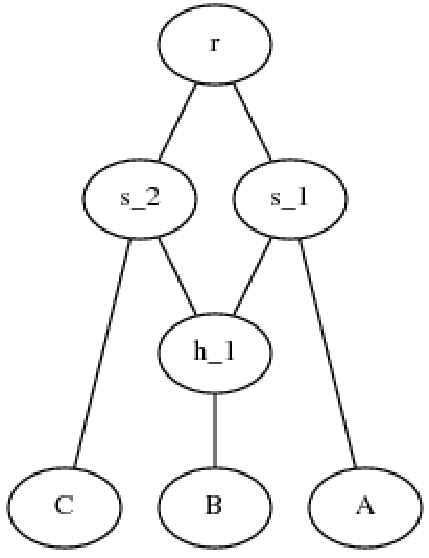
\includegraphics[height=8cm]{net_eg.pdf}
\end{center}
\indent At a hybrid node, lineages travel to either parent node with given probabilities. The parameter $\gamma$ denotes the probability of that the lineage goes to the first parent node.
Since the hybrid node has two parent nodes, the branch length needs to be specific, i.e. $t_{i}^j$ denotes the branch length from $i$ to $j$ in coalescent units.

\subsection{Method}
The coalescent model of \citet{Degnan2005} is extended to obtain the distribution of gene trees ($T$) in a given network ($W$). The network $W$ is initially reduced to a set of simpler networks ($SG(W)$) in a single step of the reduction process. By standard probability theory, we have the following:
\begin{equation*}%\PP(T|W)=\sum_{W^*\in SG(W)}\PP(T|W^*)\omega(W^*|T, W).
P(T|W)=\sum_{w^*\in SG(W)}P(T|W^*=w^*)P(W^*=w^*|W)
\label{coal_man:eqn:recursion}\end{equation*}
% $\quad\text {where }\omega(N^*|T_g=\tau, N)=\begin{cases}
% \omega_s, & \text{Case 1};\\
% \omega_h, & \text{Case 2}.
%  \end{cases}$

When each network $w^*$ is obtained from $W$ by removing an edge or a node, we will apply the recursion to reduce the networks on $W^*$ until all the simpler network structures are tree-like. The problem of obtaining gene tree probabilities from species trees has already been solved by \cite{Degnan2005}. The approach we have outlined will therefore reduce the probability of a gene tree, given a species network, into a linear combination of gene tree probabilities, given species trees.


\section{Commands:}
\subsection{Generating a list of all gene tree topologies in a taxa set}
\cm{\mbox{hybrid-coal -sp INPUT1 -gtopo [-o PREFIX]}}
%\cm{\mbox{hybrid-coal -sp INPUT1 -gtopoF OUTPUT}}
{\tt INPUT1} is a(n) (extended) Newick formatted string (see Section \ref{coal_man:coal_input}), which does not have to be a binary tree. For example, to generate a gene tree topology for the taxon set $\{A,B,C\}$:
\cm{\mbox{hybrid-coal -sp \textquotesingle(A,B,C)r;\textquotesingle  -gtopo}.}
The default setting will save the gene tree topologies to the file {\tt OUT.topo}. The file name can be specified via the option {\tt -o}, followed by {\tt PREFIX}.
%\begin{verbatim}
%(A,C),B);
%(A,(B,C));
%((A,B),C);
%\end{verbatim}

%To generate gene tree topologies for multiple lineages for the same species, e.g. for the taxon set $\{A,B,C\}$ with two lineages of species $A$, use the command:
%\cm{\mbox{hybrid-coal -sp \textquotesingle(A\_1,A\_2,B,C)r;\textquotesingle \ -gtopoF A2BC.}}
%\begin{verbatim}
%(((A_1,C),B),A_2);
%((A_1,(B,C)),A_2);
%(((A_1,B),C),A_2);
%((A_1,B),(A_2,C));
%(((A_1,B),A_2),C);
%((A_1,C),(A_2,B));
%(A_1,((A_2,C),B));
%(A_1,(A_2,(B,C)));
%(A_1,((A_2,B),C));
%((A_1,(A_2,B)),C);
%(((A_1,C),A_2),B);
%((A_1,(A_2,C)),B);
%(((A_1,A_2),C),B);
%((A_1,A_2),(B,C));
%(((A_1,A_2),B),C);
%\end{verbatim}

\subsection{Calculating gene tree probabilities of a given species network}
\cm{\mbox{hybrid-coal -sp INPUT1 [-gt INPUT2] [-o PREFIX]}}

{\tt INPUT1} is a(n) (extended) Newick formatted string (see Section \ref{coal_man:coal_input}), which can be entered through the command line or a text file.

The flags {\tt -gt} and {\tt INPUT2} are optional. {\tt INPUT2} is a Newick formatted string of a gene tree topology, which can be entered through the command line or from a text file, where users can specify several gene trees. If gene trees are not specified, {\tt hybrid-coal} will generate all possible gene tree topologies and then compute the probabilities. For example:
\cm{\mbox{hybrid-coal -sp \textquotesingle((A:1,B:1):1,C:2)r;\textquotesingle}}
will produce the following in {\tt OUT.prob}:
\begin{verbatim}
   1  ((A,C),B)   0.122626
   2  (A,(B,C))   0.122626
   3  ((A,B),C)   0.754747
\end{verbatim}

%\subsection{Generating {\tt Maple} script for the gene tree probabilities}
%{\tt hybrid-coal} can also generate {\tt Maple} script to calculate the gene tree probabilities. The option {\tt -symb} enables users to calculate the symbolic probabilities of the gene trees for analytic work. By default, the {\tt Maple} script is saved in the file {\tt maple\_prob.mw}. Users can specify the filename via the option {\tt -mapleF}.
%\cm{\mbox{hybrid-coal -sp INPUT1 [-gt INPUT2] -maple [-symb]}.}
%\cm{\mbox{hybrid-coal -sp INPUT1 [-gt INPUT2] -mapleF OUTPUT}.}


%\subsection{Generating coalescent histories for the gene tree probabilities}
%{\tt hybrid-coal} can also generate extensive \LaTeX \ code for users to study the coalescent history of a gene tree within a network.
%\cm{\mbox{hybrid-coal -sp INPUT1 [-gt INPUT2] -latex}.}
%\cm{\mbox{hybrid-coal -sp INPUT1 [-gt INPUT2] -latexF OUTPUT}.}


\subsection{Commands for other features:}
\subsubsection{Plot}
\cm{ hybrid-coal -sp INPUT -dot OUTPUT [-branch].}
{\tt hybrid-coal} uses the program {\tt dot} to generate figures. The option {\tt [-branch]} will label the branch lengths in the figure, e.g.:
\cm{hybrid-coal -sp trees/7\_tax\_sp\_nt1\_para -dot -branch.}
\begin{center}
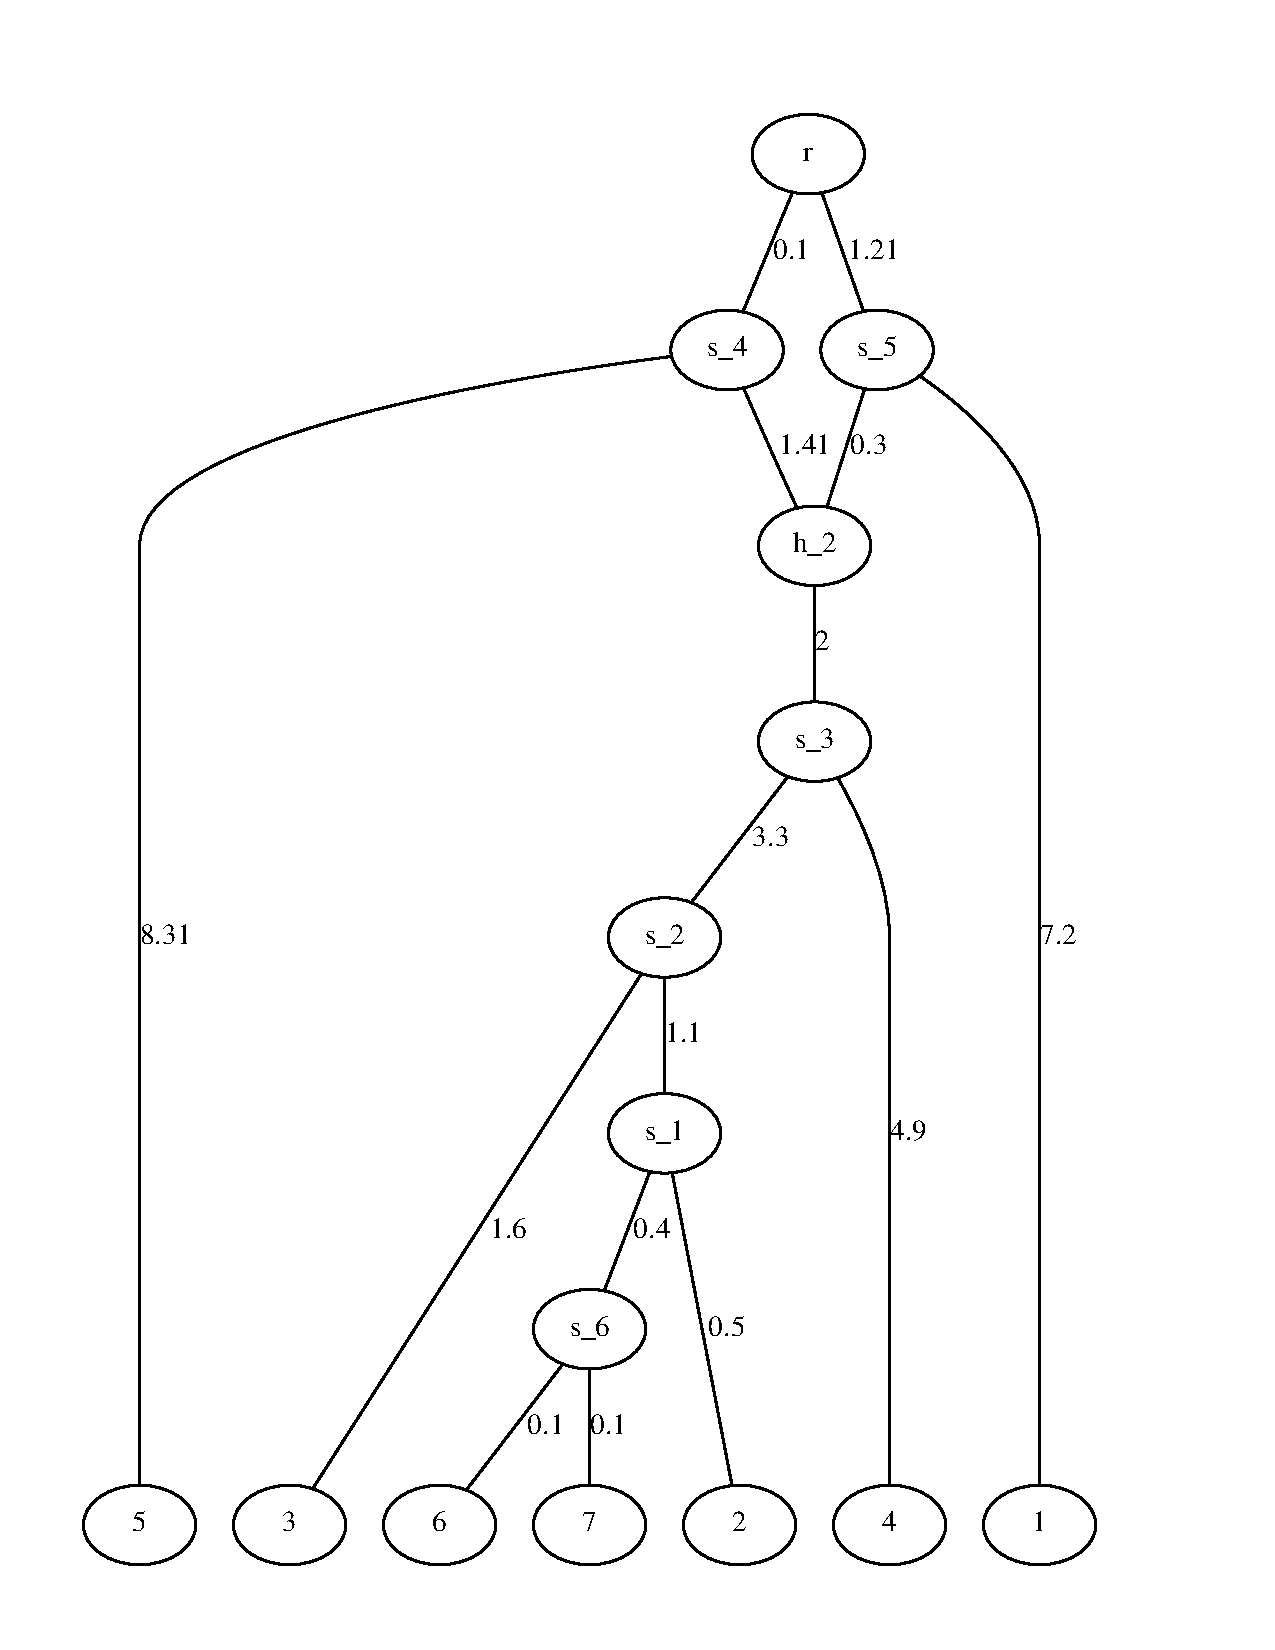
\includegraphics[width=10cm,height=10cm]{branch.pdf}
\end{center}
%If the option {\tt -dot} is used instead of {\tt -dotF OUTPUT}, the figure will be saved in the file {\tt figure.pdf} by default.

Alternatively, by replacing {\tt -dot} with {\tt plot}, {\tt hybrid-coal} can generate \LaTeX \ code for plotting a network/tree.
%If {\tt -plot} is used instead of {\tt -plotF OUTPUT}, \LaTeX \ code will be saved in the file {\tt texfigure.tex} by default.


\section{Summary of command line options}
\begin{longtable}{lp{9cm}}
{\tt -h } or {\tt -help } &  Help. List the following content.\\
{\verb -sp } {\tt INPUT} & Input the species network/tree string through the command line or from a file. Branch lengths of the {\tt INPUT} are in coalescent units.\\
{\verb -gt } {\tt INPUT} & Input the gene tree string through the command line or from a file. \\
%{\tt -latex} / {\tt -latexF} & Generate the coalescent history of a gene tree within a species network.\\
%{\tt -maple}/ {\tt -mapleF}& Generate a {\tt Maple} executable script file to calculate the gene tree probabilities of given species networks.\\
 %$\qquad${\tt -symb}& Enable the {\tt Maple} script to calculate the symbolic gene tree probabilities.\\
%{\tt -gtopo} / {\tt -gtopoF}& Generate the gene tree topologies of a given set of taxa.\\
% {\tt -sub} & \\
% {\tt -subnet}&\\
% {\tt -subtre}& \\
{\verb -o } {\tt STR } &  Specify the file name prefix of the output.\\
{\tt -plot}/{\tt -dot} {\tt [option]} & Use \LaTeX ({\tt -plot}) or {\tt Dot} ({\tt -dot}) to draw the input (defined by {\tt -sp}) network/tree.\\
% $\qquad${\tt -branch}& Branch lengths will be labelled in the figure.\\
% $\qquad${\tt -label}& Branches will be labelled by post-ordered traversal.\\
%{\tt -plotF}/{\tt -dotF} {\tt FILE}& Generated figure will be saved in {\tt FILE}.\\
\end{longtable}






\begin{thebibliography}{}

\bibitem[\protect\citeauthoryear{Brumfield and Carling}{Brumfield and
  Carling}{2010}]{Brumfield2010}
Brumfield, R.~T. and M.~D. Carling (2010).
\newblock The influence of hybrid zones on species tree inference in manakins.
\newblock In L.~L. Knowles and L.~S. Kubatko (Eds.), {\em Estimating Species
  Trees, Practical and Theoretical Aspects}, pp.\  115--127. Hoboken, NJ:
  Wiley-Blackwell.

\bibitem[\protect\citeauthoryear{Buckley, Cordeiro, Marshall, and
  Simon}{Buckley et~al.}{2006}]{Buckley2006}
Buckley, T.~R., M.~Cordeiro, D.~C. Marshall, and C.~Simon (2006).
\newblock Differentiating between hypotheses of lineage sorting and
  introgression in {New Zealand} alpine cicadas (\emph{{M}aoricicada
  {D}ugdale}).
\newblock {\em Systematic Biology\/}~{\em 55\/}(3), 411--425.

\bibitem[\protect\citeauthoryear{Cardona, Rossell, and Valiente}{Cardona
  et~al.}{2008}]{Cardona12008}
Cardona, G., F.~Rossell, and G.~Valiente (2008).
\newblock Extended {N}ewick: it is time for a standard representation of
  phylogenetic networks.
\newblock {\em BMC Bioinformatics\/}~{\em 9\/}(532-540).

\bibitem[\protect\citeauthoryear{Degnan and Salter}{Degnan and
  Salter}{2005}]{Degnan2005}
Degnan, J.~H. and L.~A. Salter (2005).
\newblock Gene tree distributions under the coalescent process.
\newblock {\em Evolution\/}~{\em 59}, 24--37.

\bibitem[\protect\citeauthoryear{Holland, Benthin, Lockhart, Moulton, and
  Huber}{Holland et~al.}{2008}]{Holland2008}
Holland, B.~R., S.~Benthin, P.~J. Lockhart, V.~Moulton, and K.~T. Huber (2008).
\newblock Using supernetworks to distinguish hybridization from
  lineage-sorting.
\newblock {\em BMC Evolutionary Biology\/}~{\em 8}, 202--213.

\bibitem[\protect\citeauthoryear{Huson, Rupp, and Scornavacca}{Huson
  et~al.}{2010}]{Huson2010}
Huson, D., R.~Rupp, and C.~Scornavacca (2010).
\newblock {\em Phylogenetic Networks: Concepts, Algorithms and Applications}.
\newblock Cambridge, UK: Cambridge University Press.

\bibitem[\protect\citeauthoryear{Meng and Kubatko}{Meng and
  Kubatko}{2009}]{Meng2009}
Meng, C. and L.~S. Kubatko (2009).
\newblock Detecting hybrid speciation in the presence of incomplete lineage
  sorting using gene tree incongruence: a model.
\newblock {\em Theoretical Population Biology\/}~{\em 75}, 35--45.


\end{thebibliography}

\end{document}

